\chapter{Estado del arte}

\subsection{Códigos correctores de errores}
En toda comunicación es importante la confiabilidad de la misma, y como ningún sistema es perfecto es esperable que se produzcan errores en la transmisión que se presentan como bits erroneos detectados por el receptor. 

La idea de un código corrector de errores esta relacionada con la técnica de espectro expandido, siendo ambos métodos que ayudan a la transmisión de la información reduciendo la entropía de la información transmitida, o lo que es lo mismo, aumentando la redundancia de la información. 

La manera mas simple de corregir estos errores es usar un algoritmo de detección de errores como puede ser un Checksum, CRC o hash[CITA], e iniciar un proceso de retransmisión de la porción o trama de datos afectada. Esto posee la desventaja de ser costoso tanto en ancho de banda perdido, como en delay de transmisión. En enlaces de muy alta velocidad las elevadas tasas de retransmisiones hacen a este algoritmo sumamente ineficiente. 
Por lo que es deseable utilizar un algoritmo que pueda detectar y corregir errores basado solamente en los bits recibidos, sin utilizar retransmisiones. Esto se denomina Forward Error Correction Codes, o FEC Codes [CITA] de los cuales existen diferentes tipos de acuerdo con sus aplicación, performance y parámetros.

\subsubsection{BCH/Reed Solomon}
Los códigos BCH y Reed-Solomon son usados ampliamente en multitud de industria ya que son computacionalmente sencillos de implementar y muy eficientes desde el punto de vista de errores corregidos por bit agregado. Se basan en operaciones sobre grupos algebráicos cíclicos cuyas operaciones sobre sus símbolos dan como resultado otro símbolo válido dentro del grupo. 
Este tipo de código si bien es relativamente antiguo, es todavía utilizado en estándares de Ethernet de 10Gbps, 100Gbps y hasta 400Gbps [CITA: IEEE P802.3bj  o ``FORWARD ERROR CORRECTION FOR 400G: INITIAL THOUGHTS''] debido a su robustez, bajo over

\subsubsection{LDPC}
El esquema de corrección de errores LDPC (Low Density Parity Check) es muy utilizado actualmente debido a su gran capacidad de corrección de errores, en algunos casos muy cercana a la máxima capacidad teórica del canal.
Antes de ahondar en la descripción de este algoritmo cabe aclarar que a pesar de ser utilizado para ciertos modelos durante la primera fase de la investigación, fue descartado en la versión final por un modelo mas simple y con menos requerimientos de hardware que presenta una performance similar desde el punto de vista de corrección de errores.
Básicamente es un código lineal que utiliza una matriz de paridad grande y dispersa.
La matriz H es tal que cualquier codeword valido x cumple con $H*x=0$

\paragraph{LDPC: Generador de matriz}
La matriz generadora puede crearse facilmente si H es de la forma $[D|I]$, simplemente formando la matriz:
$$G=[I|D']$$
Donde D' es la transpuesta de la matriz D
Para la generacion de la matriz se opto por utilizar un algoritmo random y luego aplicando algunos tests, para lograr una matriz sistemática de rate entero (1/2, 1/3, etc.)
Para verificar se G genera vectores cuya matriz de paridad es H, puede verificarse que:
$$ H*G'=0 $$

Podemos definir la matriz de paridad H como una matriz de paridad que tenga mas de 3 unos por fila y una cantidad similar por columna. Buenos resultados se obtienen a partir de matrices de 200x100.
Se puede comenzar por una matriz vacía $H = 0$ del tamaño deseado, y ir agregándole unos al azar. Cierto análisis es necesario para garantizar que no se cumplan ciclos y que la cantidad de unos por columna y por fila es la deseada. De esto se encargan los algoritmos llamados evencol y evenrow.

El generador puede generar matrices de cualquier tamaño, de esta manera:

$$ ./genMatrix <width> <height> <ones per row>$$

La matriz se genera en la salida estandard. El formato es el utilizado por la libreria boost:ublas.

NOTA: La matriz siempre esta compuesta de simbolos en GF(2) (O sea, ceros y unos)

\paragraph{LDPC: encoder}

El vector inicial se toma de la entrada estandard y el codeword se emite en la salida estandard. La sintaxis es muy sencilla:

$$ ./ldpcen <matriz> < in >out $$
\paragraph{LDPC: decoder}
Si se invoca este filtro mediante el nombre decodificador, tomara el codeword de la entrada estandard, aplicara el algoritmo de belief-propagation (Hard-decision) y se emite el vector original por la salida estandard:
La diferencia radica que en nuestro caso, al ser un canal asimetrico no se permite el bit-flip de un valor cero a un valor uno, ya que es imposible que se produzca ese error.
La linea de comando es la siguiente:

$$ ./ldpcdec <matriz> <in >out $$

La conversion codeword->vector es sencilla, ya que al ser un codigo sistemático solo se necesita eliminar la parte del vector que representa la paridad añadida.

Se generaron muchas matrices, desde 256x128 hasta matrices muy grandes de 10000x5000, pero el tiempo de decodificacion crece enormemente para matrices grandes.

\paragraph{LDPC: optimizacion}

Debido a la naturaleza iterativa del decodificador ldpc, pronto se convirtio en el cuello de botella de la simulacion. Para acelerar el sistema, se opto por realizar la siguiente optimizacion:
LDPC consta basicamente de varios loops, dentro de los cuales se accede a la matriz de paridad, y a otras matrices que acumulan datos intermedios. Primeramente la implementacion fue realizada como mencionamos utilizando boost:ublas, pero luego se comprobo que una implementacion utilizando arrays de C era hasta 3 veces mas rapida.
Luego se procedio a realizar un algoritmo de ``unrolling'' de estos loops, generando codigo especifico a una matriz dada, sin ningun tipo de loop. Obviamente este codigo es mucho mas grande, pero la aceleracion provista es aun mayor, del orden de 8 veces mas rapido que en implementaciones iniciales.
La manera de invocar el generador de codigo es la siguiente:

$$ ./genLdpcDecoder matriz  > decodeGen.h $$

El archivo generado decodeGen.h es el decodificador especifico para la matriz dada. Este header de C es luego incluido desde el decodificador ldpcenc.cpp y compilado. Al ser generalmente un archivo de un megabyte para una matriz pequeña de 1024x512, el proceso de compilacion el largo y requiere de mucha memoria.
Por otra parte, no se optimizo el proceso de codificacion ldpc, ya que consiste solo de una multiplicacion de un vector por una matriz, y es una de las tareas en la que boost:ublas es especialmente eficiente.


\subsubsection{Viterbi/Convolucional}

\subsection{Espectro ensanchado}
\label{espectroensanchado}
El espectro ensanchado, Spread Spectrum o CDMA es una técnica donde se utiliza mucho mas espectro del medio de transmisión que el necesario para la transmisión correcta de los datos.
Los origines datan del 1900, cuando Nicola Tesla patentó el concepto de \textit{"Frequency hopping"}.
El spreading de la señal tiene varias ventajas:
\begin{enumerate} 
\item Resistencia al espionaje, ya que solamente las partes que conocen la señal de spreading pueden decodificar la señal original
\item Resistencia contra interferencias de banda angosta (No a interferencias de banda ancha como el ruido térmico)
\item Capacidad de acceso múltiple. Varios usuario pueden transmitir en la misma frecuencia mientras utilicen diferentes códigos.
\end{enumerate} 
Adicionalmente, al guiarse la señal expandida con un generador pseudo-aleatorio o PRBS, se puede agregar privacidad a la comunicación haciendo imposible decodificar los datos sin tener los parámetros del PRBS.

A su vez, se puede expandir la señal en tres dominios:
\begin{enumerate} 
\item Direct Sequence (CDMA): Se expande la señal multiplicándola (XOR) con la señal de spreading, generalmente mucho más rápida. Este método es el utilizado en WiFi y WiMAX, redes 3G de celulares, etc.
\item Frecuency Hopping: La señal de spreading es utilizada para variar la frecuencia portadora de la señal original. Este método es utilizado por ejemplo en BlueTooth. (Se utiliza Adaptive Frequency Hopping, un método para evitar frecuencias con mucha interferencia)
\item Time Hopping: La señal de datos no transmite todo el tiempo, sino que sufre de un delay que depende de la señal de spreading. Este método no es muy utilizado aunque lo estudiaremos detenidamente en nuestro caso ya que es muy sencillo de implementar con los recursos de los que disponemos.
\end{enumerate} 


La desventaja de la técnica del espectro expandido, que es utilizar mucho espectro por bits transmitido, o lo que también se denomina baja densidad espectral, a veces no afecta demasiado al tener el canal una cantidad disponible de espectro mucho mayor a la utilizada. Un ejemplo de un protocolo de comunicaciones que utiliza CDMA es el protocolo WIFI, en todas sus versiones.

\subsection{Códigos de generación pseudo-aleatorio}
\label{PRNGs} 
Para que un código CDMA pueda utilizarse para obtener privacidad en la comunicación, es necesario que el parámetro a expandir, sea la frecuencia, el tiempo o el código utilizado, sea guiado o seleccionado por un generado pseudo-aleatorio o PRBS, que son algoritmos que basados en un parámetro de inicialización o semilla, son capaces de generar un stream de numeros aparentemente aleatorios, pero en realidad totalmente determinísticos. 
Es necesario que los nodos que participen de la comunicación puedan generar exactamente la misma secuencia y compartan el parámetro de generación o semilla. Esto es equivalente a lo que en criptografía se denomina un algoritmo criptográfico simétrico.
Existen muchas maneras y algoritmos de generar streams pseudo-aleatorios. Algunos algoritmos están optimizados para que su periodo (la cantidad de números en su salida antes que el patrón se repita) sea enorme, como por ejemplo el algoritmo Mersenne-twister.
Otro parámetro deseable en un PRBS es su sencillez y rapidez. Un generadores PRBS muy popular se denomina Lineal Congruential Generator y solo precisa de dos operaciones, una multiplicación y una suma.

Estos ejemplos carecen de una característica fundamental requerida en nuestro sistema: Que no se puedan predecir. Esta simple característica no es en realidad trivial ya que muchas técnicas existen para inferir datos acerca del generador PRBS, lo que supondría una falla en la seguridad de un sistema basado en dicho generador. Para evitar estos problemas existen los llamados generadores PRBS criptográficamente seguros. Como ejemplo podemos nombrar a los generadores shrinking o self-shrinking.

\subsection{Seguridad}
La propuesta es utilizar un sistema de espectro expandido con el objetivo principal de lograr la privacidad del canal al nivel físico.
Se fijaron los siguientes parámetros de seguridad:

. El sistema debe proveer confidencialidad, integridad y autenticidad de los datos.
. El sistema debe ser seguro sin importar la cantidad de clientes existentes o los datos que transmiten
. Un atacante no debe poder identificar los datos de un cliente, aunque controle todos los demas nodos de la red.

Con estos parámetros se busco el algoritmo CDMA adecuado. Las características de un sistema óptico hacen muy complejo el hardware requerido para lograr CDMA o Frequency-Hopping, pero implementar Time-hopping no presenta costo ni dificultad adicional, asi que este fue el seleccionado para la implementación de seguridad.
Varios algoritmos de asignación del time-slot fueron analizados. Se necesita que la salida de los mismos sean códigos ortogonales, o sea, deben poseer un generador capaz de crear streams pseudo-aleatorios que nunca coincidan para no generar colisiones entre los clientes. Esto no es trivial sin compartir algún tipo de información entre todos los clientes, lo que debilita la seguridad del sistema. Por ejemplo, códigos existentes llamados gold-codes permiten la generación de múltiples secuencias con baja cross-correlacion, muy util para coordinar dispositivos que comparten el medio. Pero desde el punto de vista de la seguridad, este código es trivialmente derrotado. Por ejemplo en un esquema donde un atacante controla todos los canales menos uno, el atacante podría simplemente dejar de transmitir y revelar la secuencia utilizada por la víctima, que forzosamente estara utilizando el canal restante.

Se decidió utilizar una codificación trivial: Seleccionar el time-slot de acuerdo a una secuencia criptográficamente segura estandard, totalmente independiente de los otros nodos. Es demostrable que esta decisión produce un sistema extremadamente simple y seguro. Como contrapartida, produce una cantidad muy elevada de colisiones que aumenta exponencialmente con el numero de clientes. Sin embargo, estas colisiones pueden ser corregidas mediante codificación adicional, y se logro una utilización de canal muy cercana al máximo teórico como se demostrara en la próxima sección. De echo, es en esta codificación adicional donde reside el principal aporte de esta tesis.

\subsubsection{Consideraciones de seguridad y fuerza de cifrado}\label{security}
%% extraido de dline-pub.tex
Existen varios aspectos de seguridad en un canal de comunicaciones: Autenticación, confiabilidad, confidencialidad e integridad.
El esquema presentado en esta tesis utiliza la técnica de CDMA para proveer confidencialidad, confiabilidad e integridad entre dos o mas partes, y es equivalente a un esquema de clave simétrica donde la clave compartida es utilizada para inicializar el PRNG. Aspectos adicionales tales como la autenticación puede ser implementados luego utilizando protocolos de alto nivel.
El sistema propuesto fue específicamente diseñado tomando en consideración los ataques del tipo mencionados en Ref. \cite{Shake:05}.
Como la seguridad del sistema es dependiente de su algoritmo de PRNG, se debe poner especial cuidado en la selección e implementación del mismo, que debe ser un algoritmo generador de números aleatorios para usos en criptografía, o sea criptograficamente seguro. Existen muchos algoritmos que cumplen con estas necesidades, y el PRNG propuesto en esta tesis es el llamado self-shrinking generator~\cite{Meier:94}, pero puede utilizarse cualquier otro e incluso usar diferentes algoritmos para cada cliente, con la condición que dos clientes que deseen comunicarse deben utilizar el mismo algoritmo con los mismos parámetros y claves.
Como es en el caso de otros algoritmos de clave simétrica, la clave secreta debe distribuirse de ante mano utilizando un canal seguro.

Existe una vulnerabilidad adicional inherente a sistemas ópticos dispuestos como una red en estrella: Los algoritmos de CDMA dependen en la interferencia para ofrecer confidencialidad. Sin embargo, en un sistema óptico con topología en estrella hay lugares donde poca o ninguna interferencia es presente, por ejemplo, inmediatamente a la salida de un transmisor, donde la señal de salida es alta y puede medirse y discriminarse con respecto al ruido de las demas transmisiones facilmente.
Sin embargo, los símbolos productos de la minimización del peso de hamming fueron normalizados con respecto a un dígito normal, por lo que aún si un atacante pudier escuchar y discriminar cada uno de los bits de salida, no podría decodificarlos ni inferir información alguna acerca de los bits transmitidos.

Como distintos clientes emitiend odentro de una trama se puede superponer, el atacante observara un símbolo con un HW entre 1 y W$\times$K, pero no es posible reconstruir el orden correcto de los bits sin la semilla del algoritmo generador de PRNG.

Asi mismo, muchos algoritmos de cifrado se basan en la operación de XOR (El caso del algoritmo RC4), o bien una combinación de sustituir/mezclar los datos antes de la transmision (El caso de algoritmos AES y DES), o transformaciones mas complejas (Caso RSA o algoritmos de curvas elípticas), ver Ref.~\cite{Menezes:1996:HAC:548089}.
Sin embargo, todas estas técnicas necesariamente modifican el peso de Hamming de cada símbolo en una manera que no es óptima para el esquema propuesto combinado de CDMA/Bloom-filters ya que incrementa la interferencia inter-símbolo.
Como el algoritmo propuesto se basa en CDMA del tipo time-hopping, efectivamente encripta los símbolos de entrada mientras que mantiene el deseable bajo peso de Hammings en los datos de salida, lo que se refleja menor error y en una mayor utilización del ancho de banda disponible como se muestra en la Fig.~\ref{fig_use}.

\begin{figure}[t]
  \centering
  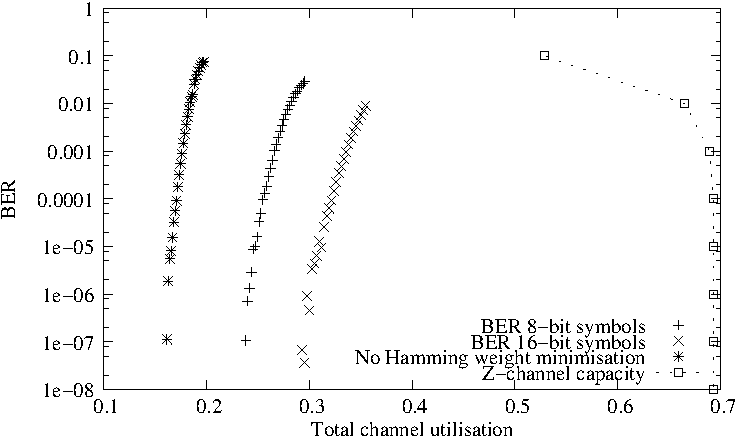
\includegraphics[width=0.48 \textwidth]{BERvsChannel} 
  \caption{Utilizacion del canal de 10 Gbps. Cada uno de los clientes (variando de 123 a 158) transmitieron 1 Gbit de datos. Notar la mejora en la utilización del ancho de banda comparada con~\cite{ortega11}.}
  \label{fig_use}
\end{figure}

En contraste con TDMA, en el esquema propuesto el atacante necesita interceptar cada una de las fibras ópticas para identificar cada usuario ya que son anonimizados luego de pasar por el hub central. Aun si el atacante puede identificar los datos, no podrá desencriptarlos sin poseer la clave correcta al estar los datos desordenados por el time-hopping y normalizado el peso de Hamming.
